\documentclass[conference]{IEEEtran}
\usepackage[T1]{fontenc}
\usepackage{amsmath,amssymb,bm,newtxtext,newtxmath}
\usepackage{graphicx,booktabs}
\usepackage[hidelinks]{hyperref}
\interdisplaylinepenalty=2500
\raggedbottom
\newcommand{\uT}{\,\mu\mathrm T}
\newcommand{\sk}[1]{[#1]_{\times}}
\begin{document}
\title{Can ordinary vessel motion calibrate a magnetometer well enough to improve marine yaw?}
\author{\IEEEauthorblockN{Ocean-IMU simulation study}}
\maketitle
\begin{abstract}
A 27-state right-invariant marine navigation filter estimates yaw from a magnetic reference acquired during startup. We isolate its independent 18-state gyro--magnetic calibration and compare constrained alternatives on paired 20-minute replays. At wave height 1.5 m the default realization gives yaw RMS of $0.720^\circ$ following and $0.460^\circ$ head. Removing magnetic noise and distortion leaves $0.178^\circ$ and $0.224^\circ$. Marine motion provides useful offset information under a restricted model. Joint gain, field and gyro-bias uncertainty leaves several affine directions poorly determined. Across four held-out draws, propagating calibration covariance changed mean yaw RMS by $+0.0007^\circ$. Withholding disturbed packets reduced it from $1.014^\circ$ to $0.855^\circ$; uninterrupted records showed essentially unchanged heading. In a separate confirmation on twelve new draws, quadrupling gyro-bias uncertainty in the learner changed sustained yaw RMS from $0.758^\circ$ to $0.751^\circ$; the paired interval included zero. Screening corrections reduced yaw RMS on clean noisy installations on two independent panels. Late application on a distorted installation increased one head-sea RMS by $1.182^\circ$.
Transporting part of each calibration-induced bearing change into the navigation attitude reduced released-record mean yaw RMS from $0.731^\circ$ to $0.711^\circ$ against the previous always-on filter.
\end{abstract}
\section{Magnetic measurement path}
The reference implementation is \texttt{bareboat-necessities/ocean-imu} at \texttt{f1424f58}. The shared TFG estimates attitude and six world motion columns with two body bias columns. One simulation adapter exercises the actual facade, acquisition, learner, invariant update and CARMA motion model.

On AtomS3R, \texttt{readMagBody\_} maps the M5 source or Bosch-trim-compensated BMM150 AUX burst to body axes. The runtime validates the saved calibration source and applies $A_0(m_{\rm raw}-b_0)$, including installation alignment when present in the fit. The sketch processes calibrated IMU data first and polls a fresh magnetic vector within 5--200 $\mu$T at 25 Hz. The IMU uses its sample clock. Optional magnetic timing metadata is diagnostic. The shared TFG sketch turns continuous correction off. The simulation injects residual distortion before the common $[y,x,-z]$ NED basis change. Its 200 Hz core and learner interpret gyro as instantaneous. The private frontend uses the separate interval-rate convention.

The shared CARMA facade uses \texttt{ProxyStartupFusion}. The private observer and wave-startup handoff establish tilt and a magnetic yaw gauge. Once live, a second independent acquisition replaces the canonical $(H,0,Z)$ reference and resets the gauge once. The CARMA wrapper schedules refinement from 90 s with a 30 s window. The startup offset fit defaults off. The legacy tilt-only offset fit solves $(I-\bar R^T\bar R)b=\bar m-\bar R^T\overline{Rm}$ with ridge and excitation checks. Its independent tilt statistics also gate the gyro-aided path.

The learner receives pre-correction magnetic samples and body gyro. Following refinement, accepted offset and inverse-matrix targets slew over 45 s. The tracker subtracts the total offset once, applies $C=A^{-1}$, and changes $H,Z$ by the difference between applied and anchored calibrations evaluated on the same statistics. It preserves canonical north. During refinement the stream is bias-corrected and the affine application is still identity. The invariant update uses $r=Rm_c-B$, $H_\phi=-\sk B$ and $R R_m R^T$. Cross-covariance transfers the update into motion and biases. The scorer accounts for declination. Navigation yaw and vessel track are unavailable to the learner.

\section{Identifiability}
Let $m_k=A f_k+b+\eta_k$, $f_k=R_k^T B$, and
\[
 f_{k+1}=\exp[-\sk{\omega_k-b_g}\Delta t]f_k .
\]
The EKF estimates $(f,b,b_g,\mathrm{vec}(A-I))$. Its first packet correlates field, offset and gain priors. Offset and gyro bias have random walks. An NIS threshold of 25, interval validation and bounds on the fitted parameters guard updates. An expanded Joseph correction preserves the covariance structure in exact arithmetic. Five hundred accepted packets qualify the fit for additional application tests.

For every $c>0$, $(A/c,cf_0)$ gives identical observations. Absolute geographic yaw also needs an external reference. With single-axis rotation the axial offset can exchange with field, and transforms commuting with all relative rotations introduce further ambiguities. Noncommuting rotations can remove exact ambiguities while leaving poor finite-record conditioning. A gain prior supplies a scale convention. Kok and Sch\"on give related inertial-aided calibration and alignment methods~\cite{kok}.

For initial-to-current field transport $U_k$, the local sensitivity at identity calibration is
\[
J_k=\left[U_k,\;-\sk{f_k}U_k\!\int_0^{t_k}\!U_s^T ds,\;I,\;(f_k^T\!\otimes I)D\right].
\]
The gain basis $D$ is orthonormal in Frobenius norm. Quotient the scalar gauge with a trace-free basis and restore the isotropic column in a separate null test. Coordinates are normalized to $1\uT$, 1 mrad/s and 1\% gain. Whiten by $0.8\uT$. In each 20 s block let $N$ contain field and gyro-bias columns and $K$ calibration columns. Stack $(I-NN^+)K$ across blocks. Its squared singular values are the profiled information eigenvalues. Free nuisance parameters in each block discard cross-block information. Using one packet in ten reduces dependence on the white-noise assumption; within-block gyro correlations can still make this optimistic. A singular value of 2 corresponds to a noise-only local standard error of half a normalized unit.

Both directions use the v1.4.0 28-foot RAO at 5 kn. The design sweep changes the yaw factor while retaining the release roll and pitch. Flat controls remove both. We compare steering of 0, 1, 3, 5 and 10 degrees, an occasional 30-degree excursion and windows of 30 to 1200 s. The release uses a 20 s steering period; the default magnetic field is $52\uT$ at $66.5^\circ$ dip. The evidence includes weak eigenvector coefficients and all singular values.

\begin{figure*}[t]\centering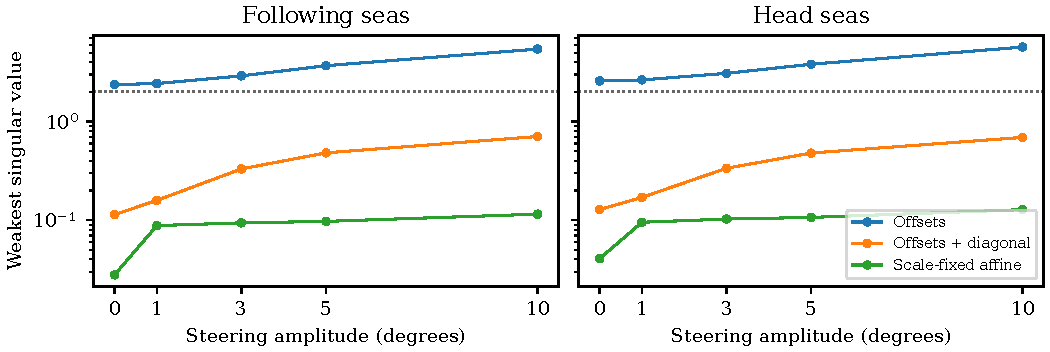
\includegraphics[width=.84\textwidth]{observability.pdf}
\caption{Weakest singular value after profiling field and gyro bias, at 1.5 m wave height.}\end{figure*}
At $\pm3^\circ$ the 1.5 m following-sea offset-only minimum is 0.42, 0.87, 1.41 and 2.91 at 30, 120, 300 and 1200 s; the head-sea values are 0.42, 0.94, 1.53 and 3.09. The weakest scale-fixed affine direction at 1200 s gives 0.094 and 0.103. Four of eleven reach 2 in each sea. The free-scale null is below $10^{-12}$. At 0.27 m only two offset-only directions in following seas and zero in head seas reach 2 in 1200 s.
\section{Controlled causes of yaw error}
\begin{table}[t]\centering\small
\caption{Yaw RMS (degrees), fixed draw, final 900 s. Off denotes the sketch calibration switch. On denotes V0.}
\begin{tabular}{lrrrr}\toprule
 & \multicolumn{2}{c}{Following} & \multicolumn{2}{c}{Head}\\
Input or intervention & Off & On & Off & On\\\midrule
known & 0.193 & 0.178 & 0.201 & 0.224 \\
ideal & 0.193 & 0.178 & 0.201 & 0.224 \\
clean & 0.206 & 0.987 & 0.209 & 0.527 \\
hard & 1.842 & 0.809 & 1.945 & 0.447 \\
diagonal & 0.252 & 0.956 & 0.182 & 0.546 \\
cross & 0.735 & 0.906 & 1.785 & 0.357 \\
alignment & 0.775 & 0.954 & 0.184 & 0.516 \\
combined & 1.909 & 0.720 & 3.375 & 0.459 \\
dip\_error & 0.285 & 0.178 & 0.262 & 0.226 \\
tilt\_kick & 0.197 & 0.184 & 0.212 & 0.233 \\
yaw\_kick & 0.516 & 0.481 & 0.327 & 0.376 \\
uncoupled & 100.321 & 86.153 & 0.850 & 0.874 \\
latency & 1.911 & 1.176 & 3.367 & 3.416 \\
burst & 2.796 & 1.836 & 3.968 & 1.529 \\
interval & 1.913 & 0.723 & 3.371 & 0.458 \\
\bottomrule
\end{tabular}\end{table}
Each arm shares the 200 Hz physical record, IMU noise, exposure schedule and start. The magnetic generator advances the same random stream when a distortion is removed. Ideal is noiseless; clean retains white magnetic noise. The off control changes only the continuous learner. The known-field arm imposes a supplied magnetic map after lock. Diagonal and symmetric cross-axis arms take components of the generated $A$; the alignment arm uses its polar rotation. The combined generator includes white noise, turn-on offset and offset random walk. The component RMS contributions cannot be added.

Default signed mean / centered RMS in following seas are $+0.529/0.489^\circ$, versus $-0.052/0.457^\circ$ in head seas. With ideal magnetic data V0 still gives signed means near $+0.075^\circ$ and $-0.136^\circ$. Replacing the acquired field by the exact map changes total RMS by under $0.001^\circ$ on each record. A $+5^\circ$ map dip perturbation and single $2^\circ$ tilt or $5^\circ$ yaw kicks following refinement probe separate sensitivities. A second executable pins the map at the actual magnetic update and injects attitude kicks at the initial live handoff. With an exact map its following/head RMS is $0.1771/0.2242^\circ$, versus $0.1780/0.2244^\circ$ for native acquisition. A persistent $+5^\circ$ dip error increases yaw RMS to $0.298/0.294^\circ$ and roll RMS to $0.944/0.674^\circ$. A $5^\circ$ handoff yaw kick gives $0.181/0.220^\circ$ late yaw RMS; a $2^\circ$ tilt kick gives $0.178/0.224^\circ$. The 80 ms latency arm delays delivered packets while retaining gyro timestamps. It substantially increases head-sea error. Switching gyro convention on this draw has a smaller effect. Device latency remains unmeasured.

Zeroing motion/nonmotion covariance blocks before every live magnetic update tests sensitivity to two-frame coupling. Following-sea displacement overflows in one intervention and exceeds 800 m RMS in the other. Its yaw RMS cannot identify a separable fraction caused by coupling. This failed diagnostic is retained in the score table.
\section{Candidate design and validation}
V0 and explicitly enabled V1 both run the gyro-aided learner. V2, V3 and V4 restrict the same EKF by zeroing prior variance in excluded affine directions; V4 retains symmetric correlated axis pairs. V5 retains the full original prior and should reproduce V0/V1. The small matrix-norm and determinant guards preclude singular corrections. V6 starts hard-only. An independent gyro and field design computes profiled information for three offsets and two trace-free diagonal gains. The weakest conditional offset information sets the applied fraction $\min(1,\lambda_b/4)$. If $\lambda_s\ge4$, both gain directions are released through a PSD prior addition that compensates the local field. The native tilt gate, startup anchor and slew remain active. A $6\uT$ predicted-vector residual quarantine advances gyro transport and covariance while withholding that packet from fitting, reference statistics and navigation. A transient leaves the earlier calibration available. A permanent field discontinuity at fixed attitude can be indistinguishable from a changed installation. Autonomous recovery from permanent interference remains unvalidated.

Development uses two joint sensor/installation draws (13, 29) on JONSWAP and both directions. The existing affine model has the lowest mean yaw RMS (0.929 degrees over 12 cells) among the baseline and constrained alternatives. V7 carries this prior. For $z=C(m-b)$ the calibration error Jacobian is $J_b=-C$, $J_{A_{:j}}=-z_j C$. Before the incoming packet the sensor-only prediction supplies a nominal vector. V7 uses
\[
 R'_m=C R_m C^T+J P_{\rm cal}J^T+dd^T
\]
where $d$ is the difference between posterior and slewed corrections on that forecast. This retains bias/gain covariance and the navigation tuning already present in $R_m$. The reference and learner share earlier observations with navigation. Temporal correlations and uncertain anchor/attitude cross-covariances are absent from this per-packet approximation. V8 adds packet quarantine to V7. A supplementary development arm retains V6 with covariance adjustment.

The holdout uses four independent joint sensor/installation draws (101, 307, 1009, 2027). Each has both directions and four PM--Stokes conditions: 0.27 m clean at $45^\circ$ dip, 1.5 m combined at $66.5^\circ$, 8.5 m combined at $76^\circ$, and 4 m with a ten-second interference burst at $55^\circ$. Dip and sea height are coupled in the panel. Paired stress cases include 1600 rpm engine vibration, an unmodeled 1 m installation offset, isolated outliers, delay, a rebuilt low--high--low round trip, weak steering and a larger turn. The full-rate estimator supplies the scores. Plots use uniform summary epochs and the repository figure decimator.
\begin{table*}[t]\centering\small
\caption{Held-out yaw RMS and paired change from V0. Intervals use four independent draw means and three Student degrees of freedom.}
\begin{tabular}{lrrrrrr}\toprule
Method & Mean (deg) & Change (deg) & Change (\%) & 95\% interval (deg) & Improved/worse & Worst increase (deg)\\\midrule
Sketch opt-out & 3.915 & +2.901 & +286.2 & [-2.22, +8.03] & 12/20 & +14.78 \\
Replay default & 1.014 & +0.000 & +0.0 & [+0.00, +0.00] & 0/0 & +0.00 \\
Existing enabled & 1.014 & +0.000 & +0.0 & [+0.00, +0.00] & 0/0 & +0.00 \\
Hard iron & 1.477 & +0.463 & +45.7 & [-0.49, +1.42] & 12/20 & +2.90 \\
Diagonal & 1.475 & +0.461 & +45.5 & [-0.47, +1.39] & 12/20 & +2.92 \\
Symmetric & 1.451 & +0.437 & +43.1 & [+0.34, +0.53] & 8/24 & +2.60 \\
Full affine & 1.014 & +0.000 & +0.0 & [+0.00, +0.00] & 0/0 & +0.00 \\
Selective & 3.186 & +2.172 & +214.3 & [-1.70, +6.04] & 12/20 & +10.35 \\
Affine + covariance & 1.014 & +0.001 & +0.1 & [-0.01, +0.01] & 16/16 & +0.03 \\
V7 + quarantine & 0.855 & -0.158 & -15.6 & [-0.22, -0.10] & 22/10 & +0.02 \\
\bottomrule
\end{tabular}\end{table*}
\begin{table*}[t]\centering\small
\caption{Means of per-record held-out scores. Signed yaw can cancel across tracks.}
\begin{tabular}{rrrrrrrr}\toprule
Arm & Signed yaw & Centered yaw & Roll & Pitch & 3-D disp. (m) & Gyro bias (mrad/s) & Acc. bias (m/s$^2$)\\\midrule
-1 & -0.611 & 0.678 & 0.245 & 0.242 & 0.175 & 0.144 & 0.060 \\
0 & 0.037 & 0.759 & 0.245 & 0.244 & 0.153 & 0.176 & 0.060 \\
1 & 0.037 & 0.759 & 0.245 & 0.244 & 0.153 & 0.176 & 0.060 \\
2 & -0.106 & 0.779 & 0.245 & 0.244 & 0.155 & 0.182 & 0.060 \\
3 & -0.115 & 0.782 & 0.245 & 0.244 & 0.155 & 0.182 & 0.060 \\
4 & 0.313 & 0.753 & 0.245 & 0.243 & 0.155 & 0.175 & 0.060 \\
5 & 0.037 & 0.759 & 0.245 & 0.244 & 0.153 & 0.176 & 0.060 \\
6 & -0.489 & 0.635 & 0.244 & 0.241 & 0.167 & 0.128 & 0.059 \\
7 & 0.036 & 0.762 & 0.245 & 0.244 & 0.153 & 0.176 & 0.060 \\
8 & 0.031 & 0.578 & 0.244 & 0.242 & 0.153 & 0.158 & 0.060 \\
\bottomrule
\end{tabular}\end{table*}
\begin{figure*}[t]\centering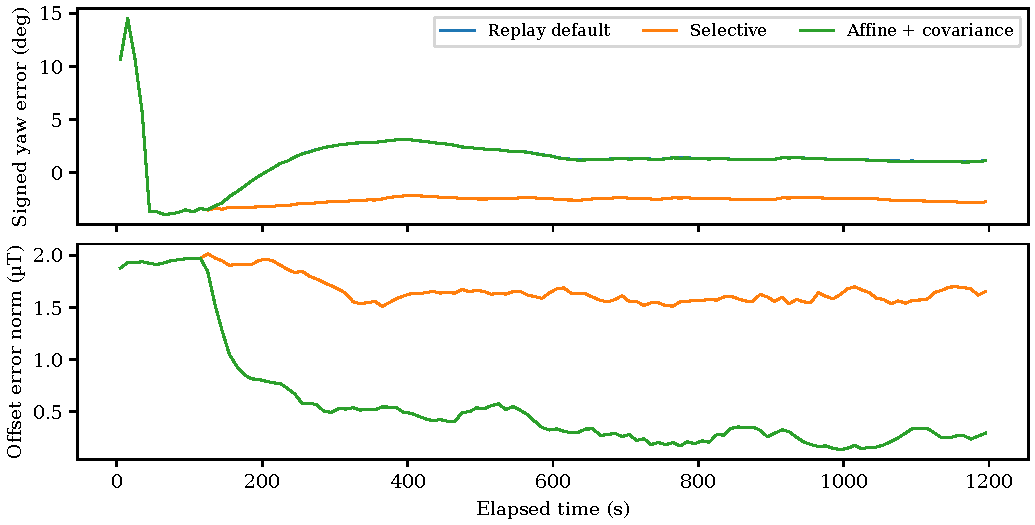
\includegraphics[width=.80\textwidth]{convergence.pdf}
\caption{Following-sea 4 m development record, draw 13. Signed yaw error and applied hard-iron error. Each yaw point summarizes five seconds.}\end{figure*}
\begin{figure*}[t]\centering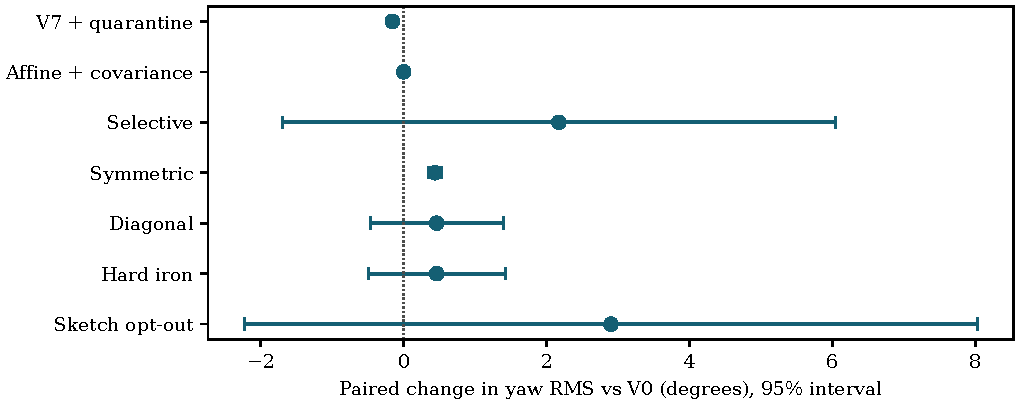
\includegraphics[width=.75\textwidth]{paired.pdf}
\caption{Held-out uncertainty across independent sensor draws. Conditions sharing a draw do not provide independent replicates.}\end{figure*}
\section{Held-out and stress results}
V0, V1 and V5 produced identical navigation and calibration scores in every paired cell. V0 averaged $1.014^\circ$ yaw RMS versus $3.915^\circ$ with the sketch calibration switch off. The four-draw interval for that overall contrast crossed zero. Clean controls favored the opt-out ($0.255^\circ$ versus $0.428^\circ$). On distorted, uninterrupted records the corresponding means were $6.029^\circ$ and $1.208^\circ$.

V2/V3/V4 averaged $1.477/1.475/1.451^\circ$, and V6 averaged $3.186^\circ$. V6's worst paired increase was $10.346^\circ$. With weak excitation it stays close to identity, protecting clean records but retaining large installation errors. On development data, hard-only estimation had lower matrix Frobenius error than V0 (0.0094 versus 0.0109) and higher yaw RMS (1.205 versus 0.929 degrees).

V7 changed mean yaw RMS by $+0.0007^\circ$ (95\% interval $[-0.0103,+0.0116]^\circ$). V8 reduced the mean to $0.855^\circ$, improving 22 cells and degrading 10. Its worst increase was $0.0155^\circ$. All four draw-level means improved, by $0.114$ to $0.199^\circ$. For the ten-second bursts the mean fell from $1.212^\circ$ to $0.582^\circ$. V8 quarantined all 250 injected packets in each held-out burst and zero packets in the 24 clean or uninterrupted distorted records. Clean and uninterrupted combined means were essentially unchanged. Following/head means fell from $0.995/1.032^\circ$ to $0.817/0.894^\circ$. Mean 3-D displacement was 0.15288 m in V0 and 0.15269 m in V8; V6 increased it to 0.16682 m. The panel assigns a specified disturbance frequency that may differ from actual vessel operation.

V0 and V8 both gave mean per-axis applied offset RMS near $(0.262,0.249,0.223)\uT$. Mean posterior offset NEES was 1.51, with about 99.9\% of sampled offsets inside the nominal 95\% ellipsoid. Hard-only coverage was about 32\%. These repeated samples are correlated. The constrained model ignores multiplicative errors. We score a usable installation after 60 consecutive seconds with applied offset error below $1\uT$ and composite matrix Frobenius error below 0.03, starting at 180 s. V0/V8 qualified in 32/32 cells (median 240 s, latest 410 s); V6 qualified in 14/32. An initially good identity calibration can qualify without online learning. The first applied change has a separate score.

In the fixed-draw interference test, the maximum difference from a matched burst-free replay was $6.64/5.96^\circ$ (following/head) for V0 and $0.06/0.06^\circ$ for V8. V0 required 189/184 s after the burst before staying within $0.1^\circ$ for 10 s. V8 was already within that band. On the uninterrupted following-sea record, regression on time, 20 s steering quadratures and true roll/pitch gave a steering-harmonic amplitude of $0.0085^\circ$ for V0. Early (300--400 s) and late (1100--1200 s) signed means were $0.289^\circ$ and $1.069^\circ$. The sustained error changes more slowly than the commanded steering on this draw.

On the separate stress draw, 80 ms lag gave $4.092^\circ$ head-sea V8 RMS versus $4.094^\circ$ V0. Quarantine responds more readily to abrupt disturbances than to smooth timing error. During the larger maneuver, following/head RMS was $0.053/0.456^\circ$ for V0 and $0.051/0.452^\circ$ for V8; over the next 80 s it was $0.204/0.501^\circ$ and $0.197/0.496^\circ$. Engine and displaced-installation results also changed little. The CSVs preserve individual records, percentiles and worst regressions.

A post-hoc ablation removed the covariance adjustment while retaining the same six-microtesla gate and native calibration. Its mean yaw RMS was $0.856^\circ$; the change from V0 was $-0.158^\circ$ (four-draw interval $[-0.213,-0.103]^\circ$). All eight burst records improved and the other 24 were identical to V0. The interrupted mean was $0.581^\circ$. Mean 3-D error was 0.15269 m, with a worst paired increase of 0.00173 m. Worst paired roll RMS increased by $0.069^\circ$. Posterior matrix-error scores were unchanged. This ablation uses the native learner's qualified field prediction; the deployed sketch's opt-out cannot supply that prediction.

The successful intervention prevents rejected packets from reaching navigation and reference statistics. The trials establish no sustained calibration advantage during uninterrupted operation. We recommend retaining existing deployment defaults. A timestamped vessel or bench comparison with independent heading would be needed to quantify actual installation error, clock offset, false quarantine rate and board headroom.

\begin{figure*}[t]\centering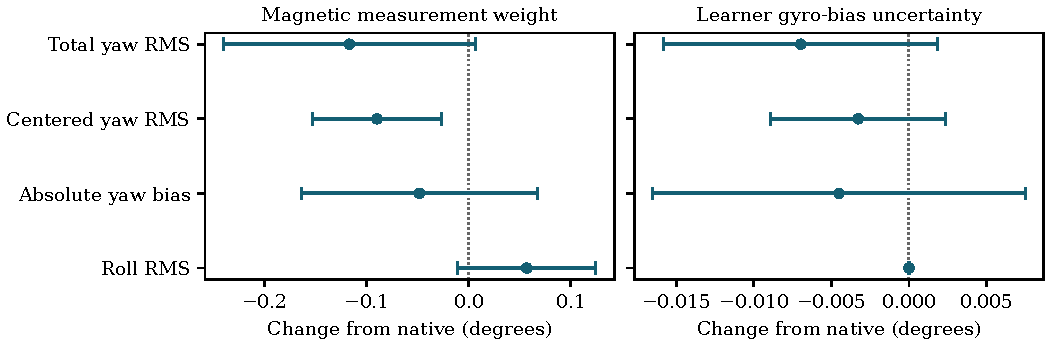
\includegraphics[width=.91\textwidth]{sustained-yaw.pdf}
\caption{Changes from the native setting on uninterrupted records. Each dot is a paired mean with its 95\% interval across independent sensor draws. Left, four draws testing stronger magnetic weight. Right, twelve further draws confirming the fourfold gyro-bias uncertainty setting. Negative changes correspond to lower error.}\end{figure*}

\section{Sustained heading without magnetic interference}
To test one alternative explanation, we changed the assumed magnetic standard deviation only after reference refinement. Each update uses the original live covariance multiplied by $k^2$. The learner, sensor packets, startup and 27-state dynamics remain identical. We scored 0.5, 1, 2 and 4 times native standard deviation on 12 uninterrupted development cells. At $k=0.5$ mean yaw RMS fell from $0.929$ to $0.871^\circ$, while roll RMS rose from $0.222$ to $0.276^\circ$. None of the three alternatives met the development requirements for yaw, absolute signed bias, roll/pitch and displacement. The lowest-yaw alternative was carried forward as a falsification test.

Four previously unused joint sensor draws (421, 829, 1609, 3517) supplied 32 paired PM--Stokes cells, all without interference, with both directions at 0.27, 1.5, 4 and 8.5 m. The 4 m cell used uninterrupted combined distortion. Mean yaw RMS fell from $0.707$ to $0.590^\circ$ ($-16.5\%$), improving 26 cells with six regressions and a worst increase of $0.138^\circ$. The paired four-draw 95\% interval for the change was $[-0.240,+0.006]^\circ$. Centered yaw RMS fell from $0.568$ to $0.479^\circ$ ($[-0.153,-0.027]^\circ$ for the change). Mean absolute within-record signed yaw bias fell from $0.324$ to $0.276^\circ$ with a change interval of $[-0.164,+0.068]^\circ$. Head-sea absolute bias improved from $0.494$ to $0.395^\circ$; following-sea bias moved from $0.154$ to $0.156^\circ$. These baseline means describe a distinct draw set.

Mean roll RMS rose from $0.180$ to $0.237^\circ$ ($+31.5\%$), with 27 regressions and a worst increase of $0.233^\circ$. Mean pitch RMS changed from $0.095$ to $0.097^\circ$ and 3-D displacement from 0.15384 to 0.15435 m. Near level attitude with field $(H,0,Z)$, the east component of a small rotation is $H\,\delta\psi-Z\,\delta\phi$, so the same magnetic residual can influence yaw and roll. This sensitivity experiment identifies a tradeoff in the full-vector update. It supplies no basis for a production-wide increase in magnetic weight.


\section{Gyro-bias uncertainty in the external learner}
Relative gyro rotation transports the local field between magnetic packets. We scaled the learner's initial gyro-bias standard deviation ($0.504$ mrad/s) and random-walk amplitude ($0.010$ mrad/s/$\sqrt{\mathrm s}$) together, keeping the navigation covariance and physical noise identical. On 12 development cells, fixing gyro bias at zero increased mean yaw RMS from $0.929$ to $9.370^\circ$. Even for clean magnetic inputs the four-cell average rose from $0.748$ to $9.812^\circ$. Across the 12 cells, mean posterior offset errors per axis grew from $(0.28,0.18,0.22)\uT$ to $(3.35,4.66,3.97)\uT$. The fitted matrix Frobenius error grew from 0.011 to 0.134. The fit can absorb angular-rate error into a spurious magnetic calibration.

At a quarter of the native standard deviations the development yaw RMS was $0.992^\circ$. A fourfold increase passed the development screen with $0.9286^\circ$ versus $0.9292^\circ$ native. Across four previously unused joint draws and 32 uninterrupted cases the fourfold setting reduced mean yaw RMS from $0.668$ to $0.656^\circ$ (25 improved, seven worsened, largest increase $0.012^\circ$). The paired 95\% change interval was $[-0.0204,-0.0026]^\circ$. Following/head means fell from $0.625/0.711^\circ$ to $0.613/0.699^\circ$. Mean absolute within-record bias changed by $-0.0126^\circ$ with interval $[-0.0260,+0.0007]^\circ$. Mean roll changed by $+0.00007^\circ$ and mean 3-D displacement by $-0.000007$ m.

We fixed the factor at four and repeated the comparison on 12 further independent sensor/initialization draws, eight physical conditions per draw. On these 96 pairs, mean yaw RMS was $0.7577^\circ$ native and $0.7507^\circ$ with the wider prior ($-0.92\%$). The draw-paired interval for the change was $[-0.0158,+0.0019]^\circ$. Fifty-three cells improved, 43 worsened and the largest increase was $0.044^\circ$. Mean absolute yaw bias changed from $0.5243^\circ$ to $0.5197^\circ$ (interval for the change $[-0.0165,+0.0075]^\circ$). Eight of the twelve draw-level total yaw means improved. Following/head yaw means moved from $0.7876/0.7277^\circ$ to $0.7771/0.7242^\circ$. On clean controls yaw rose from $0.4339$ to $0.4356^\circ$; on distorted records it fell from $0.8656$ to $0.8557^\circ$. Mean roll RMS changed by less than $0.00001^\circ$, mean 3-D displacement by $-0.000016$ m.

The seven stress fixtures in both directions averaged $1.0796^\circ$ native and $1.0786^\circ$ with the wider prior on their shared draw. The larger turn in head seas regressed from $0.753$ to $0.901^\circ$; both weak-steering records improved by about $0.033^\circ$. These results support retaining gyro bias in the external learner. Widening both its priors together failed the independent confirmation criteria for sustained yaw. The trials do not separate the initial bias variance from its random-walk rate.

\section{When does an installation need online correction?}
We crossed three magnetic inputs with three application policies on eight fresh joint draws. Each draw used all four PM--Stokes height/dip pairs in both directions. The ideal fixture supplies the exact body magnetic vector. The clean fixture adds white packet noise. The distorted fixture also includes the installation matrix, turn-on offset and offset random walk. Every arm consumes the same sensor random draws and uses the ordinary gyro, accelerometer and startup. Differences between fixtures therefore compare the indicated magnetic changes under matched motion and inertial errors.

The third policy (V11) lets the external estimator learn from the first eligible packet. It initially holds the applied correction at identity and zero offset. At five-second intervals it evaluates the estimated change in the noiseless field at the last posterior,
\[
 d=(\hat A-I)\hat f+\hat b,\qquad
 D=[\hat A-I,\ I,\ 0,\ \hat f^T\!\otimes I].
\]
It releases the native slew after three consecutive valid checks with $d^T(DPD^T)^{-1}d>16.27$, using all field, offset and matrix cross-covariances. The threshold and persistence were fixed before these replays. The repeated posterior scores are correlated, so the threshold serves as a decision rule and has no assigned record-level false alarm probability. After release the learner follows the usual application policy for the remainder of the record.

Across the 64 matched conditions, native learning reduced mean yaw RMS on distorted inputs from $3.341$ to $0.898^\circ$ (paired 95\% change interval $[-3.717,-1.170]^\circ$). On clean, noisy inputs it increased yaw RMS from $0.469$ to $0.765^\circ$ ($[+0.108,+0.484]^\circ$). With learning disabled, white packet noise changed the ideal-input mean by only $+0.001^\circ$. With learning enabled, the same noise changed it by $+0.278^\circ$. The within-draw difference of those two effects was $+0.277^\circ$ ($[+0.068,+0.485]^\circ$). White packet noise can therefore create a sustained heading penalty through online calibration even with no true offset or gain error. Residual yaw with ideal packets and learning disabled averaged $0.468^\circ$, reaching $0.984^\circ$ on the 8.5 m/$76^\circ$ condition. Height and inclination vary together in this panel.

V11 withheld the correction throughout all 64 clean noisy records, reducing mean yaw RMS from $0.765$ to $0.469^\circ$ relative to V0 ($-38.7\%$). On distorted records V11 released in 62/64 cases, at a median of 65 s among releases. Mean yaw RMS moved from $0.898$ to $0.907^\circ$ (paired change $+0.009^\circ$, interval $[-0.042,+0.061]^\circ$). Both missed releases were in 0.27 m waves. The worst regression also occurred in that sea, on a different record. Release at 745 s raised the head-sea RMS from $0.541$ to $1.724^\circ$. Delaying until the distortion is well resolved can leave a real heading error in place for much of the scoring window.

\begin{figure*}[t]\centering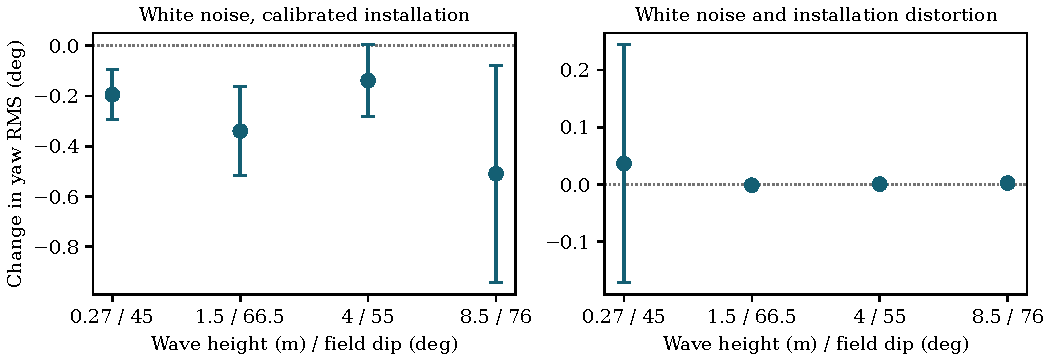
\includegraphics[width=.93\textwidth]{installation-screen.pdf}
\caption{Change in yaw RMS when applying the installation screen instead of always-on calibration. Each point averages the paired effects across both directions within each of eight independent draws. Bars show two-sided 95\% intervals across those draws. The vertical scales differ.}\end{figure*}

\begin{table}[t]\centering\footnotesize
\caption{Mean yaw RMS in degrees for opt-out, native continuous calibration and screened application. The last column counts records in which V11 released the correction.}
\begin{tabular}{llrrrr}\toprule
Panel & Input & Off & Native & V11 & Released\\\midrule
Four seas & Ideal & 0.468 & 0.487 & 0.468 & 0/64 \\
Four seas & Clean & 0.469 & 0.765 & 0.469 & 0/64 \\
Four seas & Distorted & 3.341 & 0.898 & 0.907 & 62/64 \\
0.27 m & Ideal & 0.377 & 0.368 & 0.377 & 0/32 \\
0.27 m & Clean & 0.392 & 0.624 & 0.392 & 0/32 \\
0.27 m & Distorted & 3.433 & 0.778 & 0.801 & 32/32 \\
\bottomrule
\end{tabular}\end{table}

We then fixed the 0.27 m record, crossed magnetic dips of $45^\circ$ and $76^\circ$ in both directions, and repeated the nine arms on eight independent new draws (288 replays). On 32 clean noisy records the screen again withheld every correction. Mean yaw RMS fell from $0.624$ to $0.392^\circ$ relative to V0 (paired change $-0.232^\circ$, interval $[-0.448,-0.016]^\circ$). The interval for the change in absolute within-record signed bias included zero on both panels. On distorted weak-wave records the screen released in all 32 cases, at median 112.5 s. Mean yaw RMS moved from $0.778$ to $0.801^\circ$ ($+0.023^\circ$, interval $[-0.011,+0.057]^\circ$). Even with eventual detection, a 375 s release raised one head-sea RMS from $0.226$ to $0.633^\circ$. Across the distorted cases the maximum paired increases in roll and pitch RMS stayed below $0.001^\circ$ on both panels. These results support screening as a way to protect an already calibrated installation in simulation. They give no sustained-yaw advantage over native learning when actual distortion is present. The release delays and absence of vessel trials limit deployment.

The fixed stress draw covered engine vibration, displaced mounting, magnetic latency, outliers, a low--high--low sea transition, weaker steering and a larger turn in both directions. The screen released between 40 and 80 s in all 14 records, before the ordinary post-refinement correction became eligible. All 14 sustained yaw scores matched V0. These records exercise the early-release path and give limited information about disturbances that start while a correction is still withheld.


\section{Integration in the navigation filters}
The calibration runs outside the navigation state. The filter feeds raw magnetic measurements to the learner and checks the preceding posterior every five seconds. Three successive distortion detections permit the ordinary calibration slew. The runtime option is shared by the proxy-startup filters and the standalone TFG. Seven AtomS3R sketches expose the option at build time.

\begin{table*}[t]\centering\small
\caption{Mean yaw RMS in degrees across 16 released records per filter, each scored over its last 900 seconds with the earlier 45-second calibration response. The last column gives the number of complete quality-gate passes out of 16 for each mode in column order.}
\begin{tabular}{lrrrr}\toprule
Filter & Off & Always on & Screened & Gate passes (off/on/screened)\\\midrule
TFG shared-mode CARMA & 2.732 & 0.731 & 0.786 & 0/16/12 \\
QMEKF shared-mode CARMA & 2.735 & 0.742 & 0.798 & 0/16/12 \\
Tangent shared-mode CARMA & 2.738 & 0.736 & 0.791 & 0/16/12 \\
TFG CARMA & 2.738 & 0.735 & 0.790 & 0/16/12 \\
QMEKF CARMA & 2.741 & 0.747 & 0.802 & 0/16/12 \\
OU-II & 2.830 & 0.816 & 0.865 & 0/16/12 \\
OU-III & 2.776 & 0.759 & 0.813 & 0/16/12 \\
TFG & 2.576 & 0.684 & 0.723 & 0/16/10 \\
\end{tabular}\end{table*}

On TFG shared-mode CARMA the screened policy lowered mean yaw RMS by 71\% relative to the saved-calibration sketch policy. Screening beat off on all 16 records and tied always on at the reported precision on all 12 records above $0.27$~m. Mean following-sea yaw RMS was $0.7605^\circ$ screened and $0.7602^\circ$ always on. In head seas it was $0.812^\circ$ screened and $0.702^\circ$ always on. On the two $0.27$~m head-sea records screening increased yaw RMS by $0.429^\circ$ and $0.448^\circ$. The four screened runs that exceeded the gyro-bias limit all had $0.27$~m waves. On the two head-sea records, gyro-bias RMS rose 25--27\% relative to always on. These records use the replay installation model. The independent clean-input panels above cover the complementary case where residual installation distortion is absent. The sketch feature remains opt-in pending device measurements.

\section{Calibration and heading response in the TFG shared-mode filter}
The calibration slew changes the body-frame bearing delivered to navigation even if the vessel and the sampled field are stationary. Assigning the entire change to the magnetic innovation can also move the gyro-bias estimate. The TFG shared-mode configuration now slews the correction over 60~s. For each applied step, let $u=R K_{\rm old}(m-b_{\rm old})$ and $v=R K_{\rm new}(m-b_{\rm new})$, computed from the same raw packet $m$ and predicted attitude $R$. Before the ordinary magnetic update, we apply a world-vertical rotation of
\[
  0.2\,\operatorname{atan2}(v_xu_y-v_yu_x,\;v_xu_x+v_yu_y).
\]
The transport requires a finite input, a positive horizontal dot product above the squared minimum field threshold, and a corrected field norm between half and 1.5 times the reference norm. The estimator uses its existing attitude-write operation. The comparison uses the previous always-on learner with a 45~s slew and zero bearing transport. Both receive identical sensor packets.

An alternative changed the slew from 45 to 180~s at elapsed time 300~s. On the 16 released records it reduced mean yaw RMS from $0.731^\circ$ to $0.626^\circ$, passing every original gate. With four new joint sensor draws its mean increased from $1.040^\circ$ to $1.109^\circ$. This sensitivity motivated the independent validation of the smaller, continuous correction.

\begin{table*}[t]\centering\small
\caption{Mean per-record yaw RMS in degrees. Independent panels contain both sea directions at three heights per draw. Paired intervals use the sensor draw as the independent unit.}
\begin{tabular}{lrrrrr}\toprule
Panel & Records & Previous & Transported & Paired change & 95\% interval on change\\\midrule
Released records & 16 & 0.731 & 0.711 & $-0.020$ & --- \\
8 fresh sensor draws & 48 & 0.959 & 0.931 & $-0.028$ & $[-0.062, +0.007]$ \\
32 fresh sensor draws & 192 & 0.789 & 0.767 & $-0.022$ & $[-0.036, -0.009]$ \\
\end{tabular}\end{table*}

Seven of eight validation draws and 22 of 32 replication draws improved. The 32-draw panel reduced mean yaw RMS in following seas from 0.831 to 0.809 degrees and in head seas from 0.747 to 0.724 degrees. The new configuration passed all 16 original production gates and all 16 legacy interval-rate gates. On production defaults, 15 of 16 records improved. The 8.5~m head-sea PM--Stokes record increased by $0.0012^\circ$. Mean gyro-bias RMS fell from 0.1150 to 0.1090~mrad/s. Mean 3-D displacement RMS was 0.14754~m for both settings. The pinned case and independent draws use the simulator's residual magnetic installation model.

\section{Numerics and embedded cost}
On Espressif GCC 14.2.0 (\texttt{esp-14.2.0\_20241119}), compiled for ESP32-S3 with \texttt{-Os}, the learner object is 1508 bytes. Its largest emitted frame is 3696 bytes in the magnetic update. The selective prototype adds a 216-byte object and at least 1168 heap bytes for two dense double matrices, plus decomposition temporaries. Its object file contains 167029 text/read-only bytes before linker garbage collection. Its largest emitted frame is 736 bytes. These measurements exclude whole-program linkage and runtime stack high-water. A 30000-packet x86 microbenchmark measured 3.23 microseconds for eight gyro predictions plus one native update and 0.077 microseconds per gate packet averaged across block solves. The separate V8 covariance/quarantine arithmetic cross-compiles to 6921 unlinked text bytes with a largest emitted frame of 1872 bytes. On the host its full-output checksum benchmark measured 1.00 microsecond of CPU time per packet. Physical board timing, peak heap and watchdog margin remain unmeasured. The dynamic double-precision gate needs a bounded-memory implementation and device measurements before an embedded trial.
\section{Reproduction}
The adjacent README gives commands. The per-cell CSVs include bias, centered and total yaw, displacement components, sensor-bias RMS, applied and posterior calibration errors, conditional information and covariance checks. Raw waves and full-rate logs are regenerable.
\begin{thebibliography}{1}
\bibitem{kok} M. Kok and T. B. Sch\"on, Magnetometer calibration using inertial sensors. \emph{IEEE Sensors Journal}, vol. 16, pp. 5679--5689, 2016. \url{https://arxiv.org/abs/1601.05257}.
\end{thebibliography}
\end{document}
